
\subsubsection{Создание базы данных}

Для хранения данных приложений была создана база данных
представляющая собой следующий набор сущностей:

пользователь конструктора;
\begin{itemize}
	\item пользователь бота;
	\item бот;
	\item группа компонентов;
	\item компонент.
\end{itemize}

Пользователь хранит логин и пароль для возможности аутентификации
его в системе.

Бот содержит такую информацию, как имя и принадлежность какому-
либо пользователю путем указания его идентификатора.

Пользователь бота содержит информацию, которая старается подробно
его описать. Сюда входят такие поля, как идентификатор телеграмма, имя,
фамилия, ник. Также для хранения текущей сессии пользователя бота
содержаться поля идентификатора компонента и контекста.

Группа компонентов содержит поля имени группы, а также поле
указания принадлежности к определенному боту. Группы позволяют
потенциально расширить возможность конструктора, введя туда компонент,
который будет отвечать за определение и вызов функций – набор
компонентов.

Компонент содержит поля типа, пути, данных, выходов,
идентификатора следующего компонента и позиции на области редактора.

ER-диаграмма представлена на рисунке~\ref{f:erd}.

\begin{figure}[ht]
	\centering
	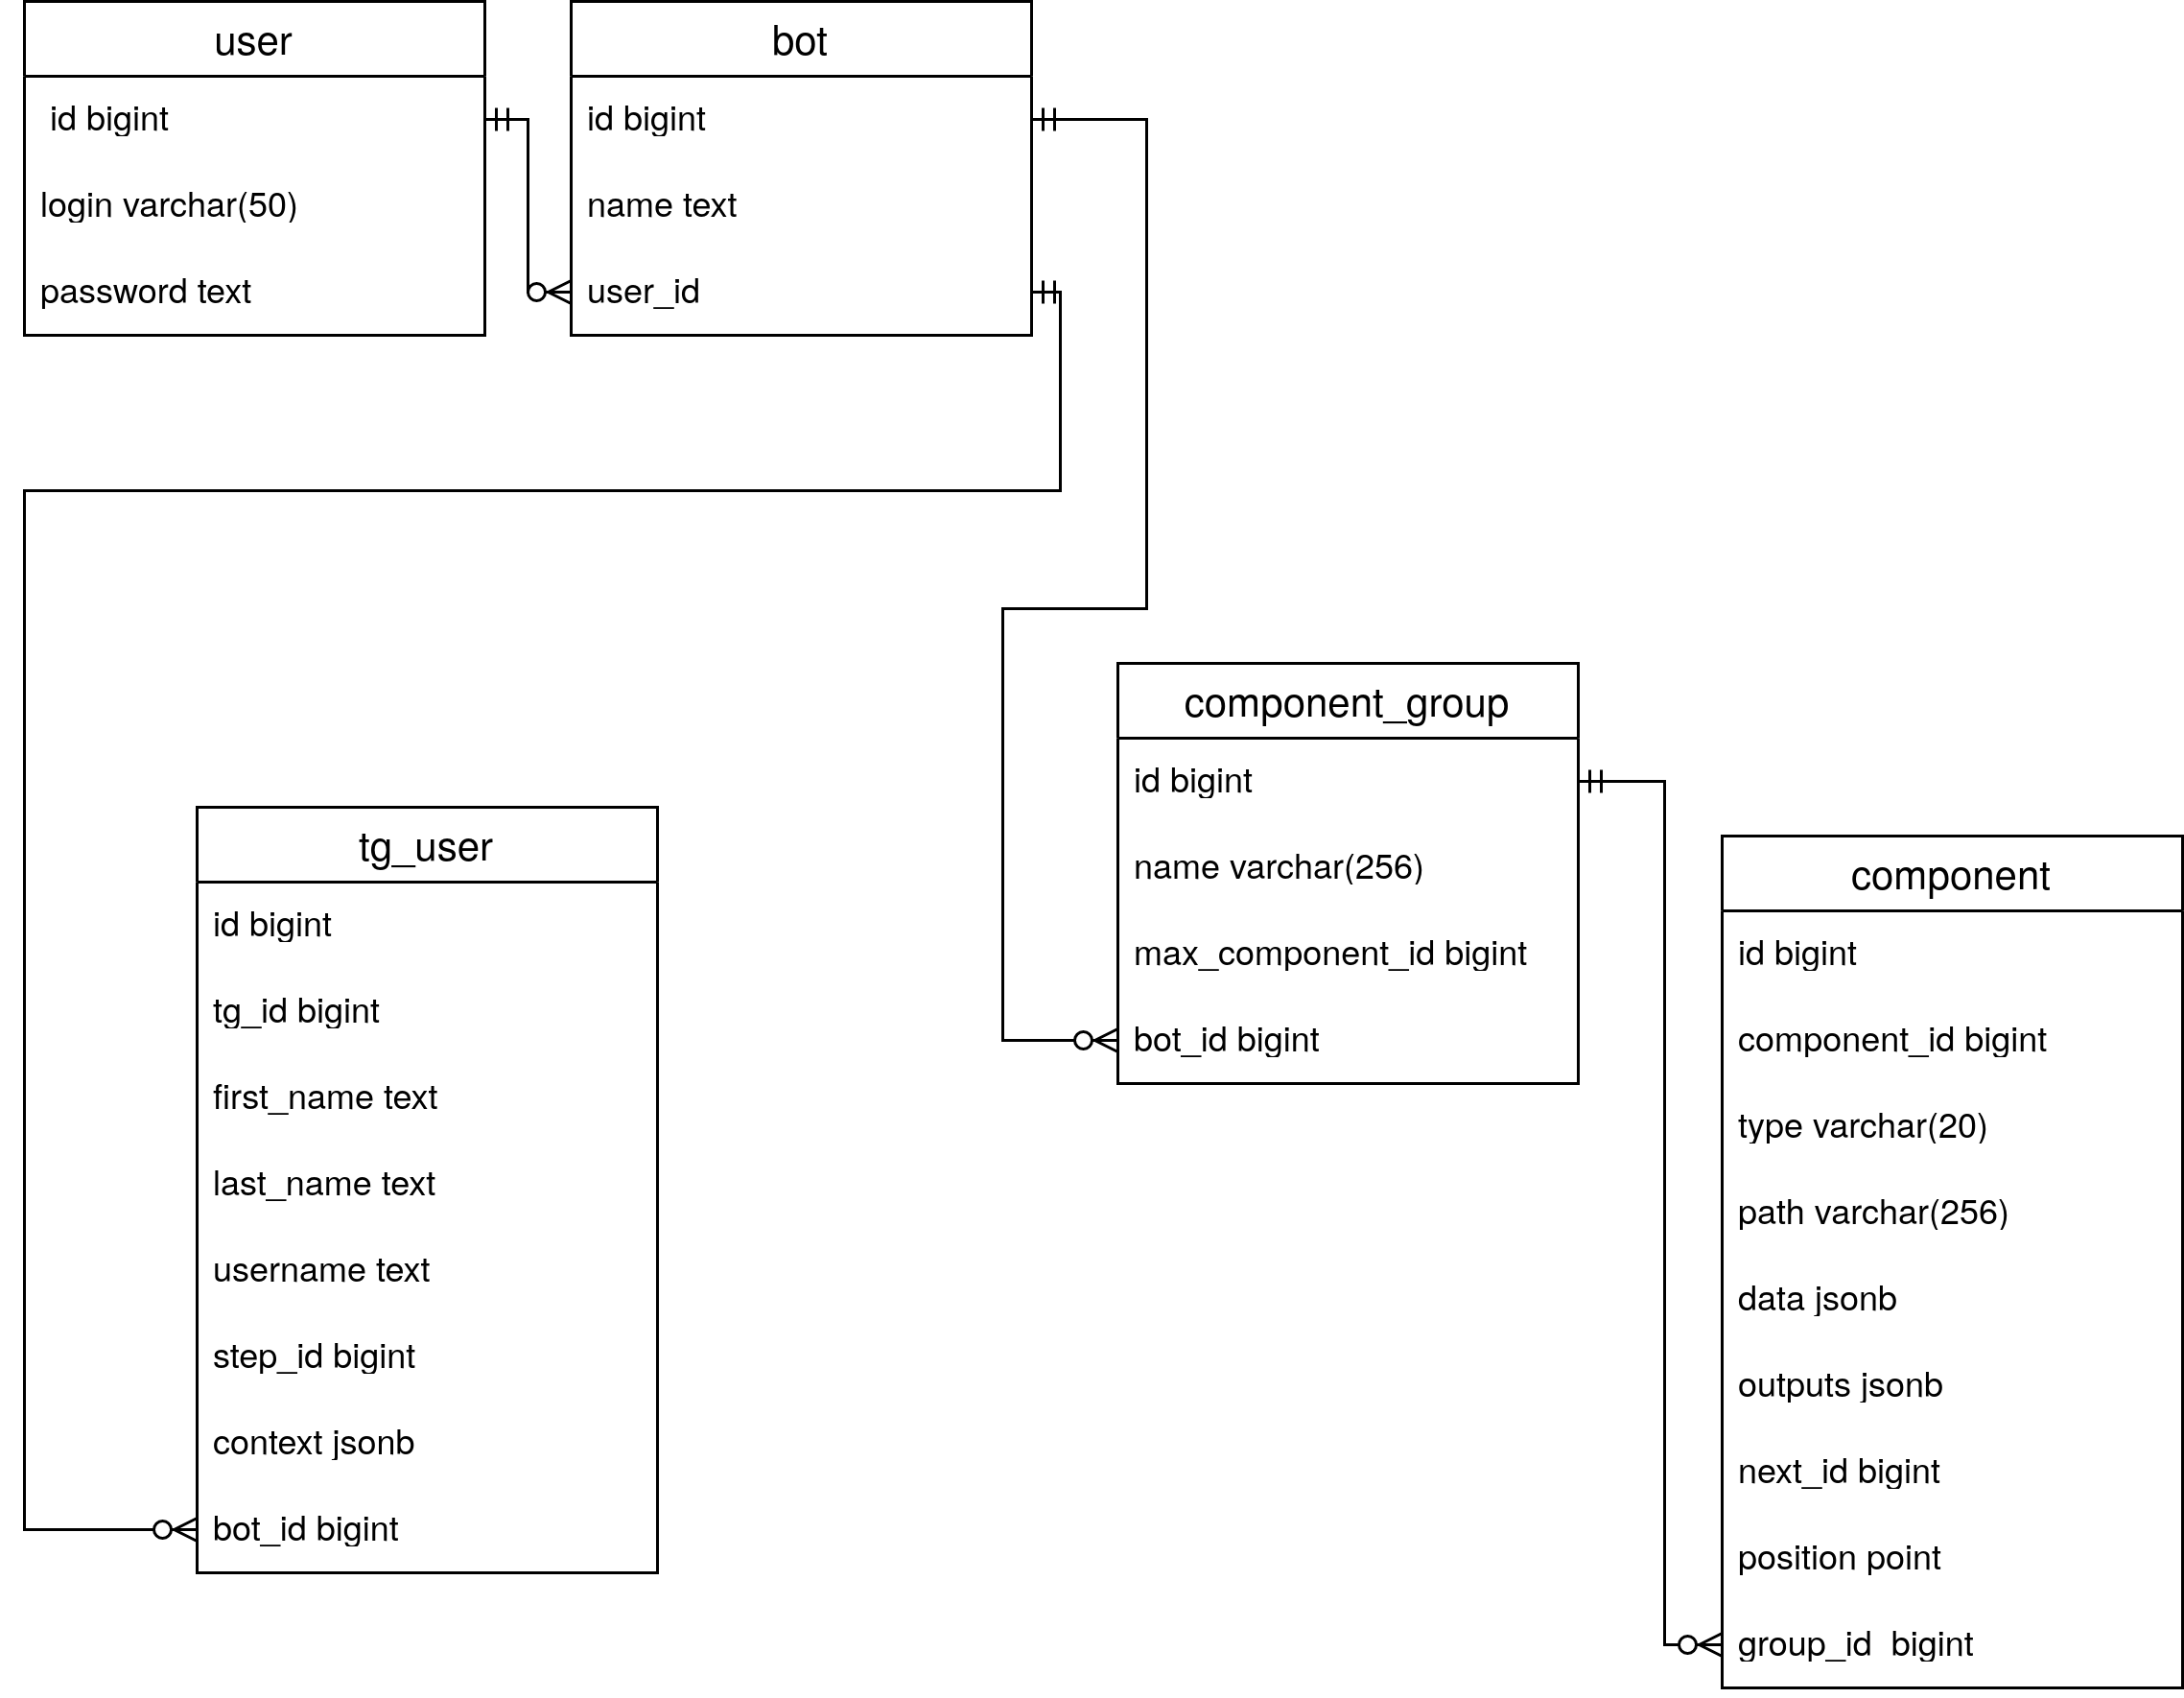
\includegraphics[width=0.95\textwidth]{db}
	\caption{Общая структура конструктора}
	\label{f:erd}
\end{figure}


